\documentclass{dlproblemset}
\usepackage{tikz}
\usetikzlibrary{positioning}
\tikzset{every picture/.style={line width=0.75pt}}

\title{Regularização}
\subtitle{Lista de Exercícios}

\begin{document}

\begin{enumerate}[1)]

    \item \textit{Label Smoothing} é uma técnica de regularização que visa diminuir a tendência de \textit{overfitting} do modelo combatendo principalmente inferências com \textit{overconfidence}. Essa técnica redefine os valores alvo da seguinte forma:
    \begin{equation*}
     \mathbf{y}^{(i)}_{ls} = (1 - \alpha)\mathbf{y}^{(i)}_{\text{oh}} + \frac{\alpha}{C}
    \end{equation*}
    \noindent onde $\mathbf{y}^{(i)}_{\text{oh}}$ é a variável alvo codificada em \textit{one-hot encoding}, $\alpha$ é a constante de \textit{smoothing} e $C$ é o número de classes do problema. Sobre \textit{Label Smoothing}, marque as alternativas verdadeiras:

    \begin{enumerate}[(a)]
	    \item Quando $\alpha=1$ a variável alvo fica distribuída uniformemente entre as classes.
	    \item Quando $\alpha=0$ a variável alvo permanece inalterada em formato \textit{one-hot encoding}.
	    \item Para encontrar o valor ideal de $\alpha$ devemos considerar a quantidade de observações no conjunto de dados.
	    \item Quando $\alpha=0$ temos a maior intensidade de \textit{smoothing}.
    \end{enumerate}
    %a, b

    \item Sobre as penalidades de regularização L1 e L2 adicionadas à função de custo, $\tilde{\mathcal{L}}(\boldsymbol{\theta}) = \mathcal{L}(\boldsymbol{\theta}) + \lambda\,\Omega(\boldsymbol{\theta})$ com $\Omega_{L1} = \|\boldsymbol{\theta}\|_1$ e $\Omega_{L2} = \|\boldsymbol{\theta}\|_2^2$, é correto afirmar que:
    \begin{enumerate}[(a)]
        \item A penalidade L2 tende a zerar exatamente alguns componentes do vetor de pesos, induzindo soluções esparsas.
        \item A penalidade L1 tende a zerar exatamente alguns componentes do vetor de pesos, induzindo soluções esparsas.
        \item A penalidade L1 equivale, na visão probabilística, a adicionar um \textit{prior} gaussiano sobre os pesos no critério de máxima verossimilhança.
        \item A penalidade L2 aumenta a magnitude dos pesos durante o treinamento para compensar o termo adicional na função de custo.
    \end{enumerate}
    %b

    \item Uma rede foi treinada com \textit{dropout}, desligando cada unidade oculta com probabilidade $p$ a cada \textit{forward pass}. Na inferência, todas as unidades permanecem ativas. Sobre o ajuste necessário nesse cenário, é correto afirmar que:
    \begin{enumerate}[(a)]
        \item As ativações devem ser multiplicadas por $p$ na inferência, restaurando a fração de unidades que era desligada durante o treino.
        \item Nenhum ajuste é necessário, pois o \textit{dropout} altera apenas o \textit{backward pass} e não muda a escala das ativações.
        \item As ativações devem ser multiplicadas por $(1-p)$ na inferência, compensando a diferença de magnitude esperada em relação ao treino.
        \item Os pesos devem ser reamostrados com variância $(1-p)$ antes da inferência, igualando a distribuição das pré-ativações à do treino.
    \end{enumerate}
    %c

    \item Demonstre que uma regularização L2 na função de custo de uma unidade com função de ativação identidade é equivalente a diminuir a magnitude do vetor de pesos antes de realizar a atualização. \textit{Dica: escreva a função de custo com o termo de regularização $||\boldsymbol{\theta}||^2$ e use essa função de custo na expressão de atualização dos pesos da descida de gradiente. Colocando o $\boldsymbol{\theta}$ em evidência ficará claro que os pesos estão sendo multiplicados por um valor na faixa $(0,1)$.}

    \item Durante o treinamento com \textit{dropout}, a ativação $a$ de uma unidade oculta é multiplicada por uma máscara binária $m \sim \text{Bernoulli}(1-p)$, onde $p$ é a probabilidade de desligamento. Resolva os itens abaixo:
    \begin{enumerate}[a)]
        \item Calcule $E[m \cdot a]$ e compare o resultado com a magnitude da ativação em inferência, quando a unidade está sempre ativa.
        \item Explique as duas formas vistas em aula de corrigir essa diferença de escala: o \textit{rescaling} determinístico em inferência e o \textit{inverted dropout} adotado como padrão por PyTorch e Keras.
    \end{enumerate}

    \item Explique o funcionamento do \textit{early stopping}: o que é monitorado durante o treinamento, qual o papel do hiperparâmetro \textit{patience} e por que a técnica tem efeito análogo ao da regularização L2. Cite também o benefício adicional que ela traz além do efeito regularizador.

    \item Durante o treinamento, uma camada de \textit{dropout} com taxa $p$ sorteia, a cada iteração, uma máscara binária com o mesmo formato da sua entrada: cada posição vale $0$ com probabilidade $p$ e $1$ caso contrário. A camada multiplica a entrada, elemento a elemento, pela máscara e multiplica o resultado por $1/(1-p)$, para que o valor esperado de cada ativação não mude (\textit{inverted dropout}).

    Considere o MLP $1 \times 2 \times 2 \times 1$ abaixo, com $\mathbf{z}^{(l)} = \mathbf{a}^{(l-1)}{\mathbf{\Theta}^{(l)}}^{\top} + \mathbf{b}^{(l)}$, ReLU nas duas camadas ocultas, saída linear e uma camada de \textit{dropout} com $p = 0{,}5$ aplicada sobre $\mathbf{a}^{(1)}$:

    \begin{center}
    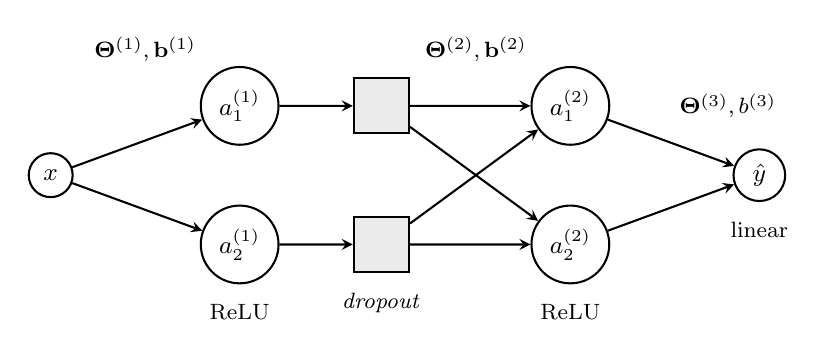
\begin{tikzpicture}[>=stealth, yscale=0.8, every node/.style={font=\small}]
        % entrada
        \node[circle, draw] (x) at (0, 0) {$x$};
        % primeira camada oculta (ReLU)
        \node[circle, draw] (a1) at (2.4, 1.1)  {$a^{(1)}_1$};
        \node[circle, draw] (a2) at (2.4, -1.1) {$a^{(1)}_2$};
        % dropout: um quadrado por unidade
        \node[rectangle, draw, fill=black!8, minimum size=7mm] (d1) at (4.2, 1.1)  {};
        \node[rectangle, draw, fill=black!8, minimum size=7mm] (d2) at (4.2, -1.1) {};
        % segunda camada oculta (ReLU)
        \node[circle, draw] (c1) at (6.6, 1.1)  {$a^{(2)}_1$};
        \node[circle, draw] (c2) at (6.6, -1.1) {$a^{(2)}_2$};
        % saída linear
        \node[circle, draw] (y) at (9.0, 0) {$\hat{y}$};
        \draw[->] (x) -- (a1); \draw[->] (x) -- (a2);
        \draw[->] (a1) -- (d1); \draw[->] (a2) -- (d2);
        \draw[->] (d1) -- (c1); \draw[->] (d1) -- (c2);
        \draw[->] (d2) -- (c1); \draw[->] (d2) -- (c2);
        \draw[->] (c1) -- (y); \draw[->] (c2) -- (y);
        % rótulos das camadas
        \node[font=\footnotesize] at (1.2, 2.0)  {$\mathbf{\Theta}^{(1)}, \mathbf{b}^{(1)}$};
        \node[font=\footnotesize] at (5.4, 2.0)  {$\mathbf{\Theta}^{(2)}, \mathbf{b}^{(2)}$};
        \node[font=\footnotesize] at (8.6, 1.1) {$\mathbf{\Theta}^{(3)}, b^{(3)}$};
        \node[font=\footnotesize, below=0.12cm of a2] {ReLU};
        \node[font=\footnotesize, below=0.12cm of d2] {\textit{dropout}};
        \node[font=\footnotesize, below=0.12cm of c2] {ReLU};
        \node[font=\footnotesize, below=0.12cm of y]  {linear};
    \end{tikzpicture}
    \end{center}

    Os parâmetros, a instância de treino e a máscara sorteada nesta iteração são
    \[
    x = 2, \quad
    \mathbf{\Theta}^{(1)} = \begin{bmatrix} -1 \\ 2 \end{bmatrix}, \quad
    \mathbf{b}^{(1)} = \begin{bmatrix} 3 & 1 \end{bmatrix}, \quad
    \mathbf{\Theta}^{(2)} = \begin{bmatrix} 3 & 0{,}5 \\ -2 & -2 \end{bmatrix}, \quad
    \mathbf{b}^{(2)} = \begin{bmatrix} 1 & 0 \end{bmatrix},
    \]
    \[
    \mathbf{\Theta}^{(3)} = \begin{bmatrix} -1 & -3 \end{bmatrix}, \quad
    b^{(3)} = 1, \quad
    p = 0{,}5, \quad
    \text{máscara} = \begin{bmatrix} 1 & 0 \end{bmatrix}.
    \]
    Qual é a saída $\hat{y}$ da rede nesta iteração de treinamento?

    \begin{enumerate}[(a)]
        \item $\hat{y} = -5{,}5$
        \item $\hat{y} = -6$
        \item $\hat{y} = -3$
        \item $\hat{y} = -1{,}5$
        \item $\hat{y} = -5$
        \item $\hat{y} = 6$
        \item $\hat{y} = 0$
        \item $\hat{y} = -12$
    \end{enumerate}
    %b

\end{enumerate}

\newpage

\subsection*{Gabarito}
\color{blue}
\begin{enumerate}[1)]

    \item a, b. Basta substituir na fórmula: com $\alpha=1$ o termo \textit{one-hot} é anulado e sobra $\frac{1}{C}$ em todas as classes, o alvo uniforme (a); com $\alpha=0$ a fórmula devolve o alvo \textit{one-hot} original, sem nenhuma suavização (b), o que também mostra que (d) está invertida. O valor de $\alpha$ (c) é um hiperparâmetro de intensidade da suavização, não uma função da quantidade de observações do conjunto.

    \item b. A penalidade L1 empurra componentes pequenos até exatamente zero (os vértices do losango da bola L1 ficam sobre os eixos), induzindo esparsidade; a L2 encolhe as magnitudes sem zerá-las, o que exclui (a). Na visão probabilística, L1 corresponde a um \textit{prior} laplaciano e L2 ao gaussiano, o que exclui (c); e ambas diminuem a magnitude dos pesos, o contrário de (d).

    \item c. Durante o treino cada unidade fica ativa com probabilidade $1-p$, então a magnitude esperada das ativações que as camadas seguintes aprenderam a receber é $(1-p)$ vezes a magnitude sem \textit{dropout}. Com todas as unidades ativas na inferência, multiplicar as ativações por $(1-p)$ restaura essa escala. Multiplicar por $p$ (a) corrige na direção errada, e (b) ignora que o \textit{dropout} altera a escala do próprio \textit{forward}.

    \item $\boldsymbol{\theta}_{(t+1)}=(1 - 2\eta \lambda)\boldsymbol{\theta}_t - \eta\nabla_{\boldsymbol{\theta}} J$, onde $\lambda$ é a constante de regularização L2.

    \item
    \begin{enumerate}[a)]
        \item Como a máscara é independente do valor da ativação e $E[m] = 1-p$, temos $E[m \cdot a] = E[m]\,a = (1-p)\,a$. Em inferência a unidade está sempre ativa e produz $a$, ou seja, uma magnitude $\frac{1}{1-p}$ vezes maior do que a magnitude esperada que as camadas seguintes viram durante o treino.
        \item \textit{Rescaling} determinístico: multiplicar as ativações por $(1-p)$ na inferência, trazendo a escala de teste para a escala esperada do treino. \textit{Inverted dropout}: dividir as ativações por $(1-p)$ já durante o treino, de modo que a magnitude esperada fique igual à de inferência e nenhum ajuste seja necessário ao testar; é o padrão em PyTorch e Keras.
    \end{enumerate}

    \item O \textit{early stopping} monitora o desempenho da rede em um conjunto de validação ao longo do treinamento e interrompe o processo antes que a \textit{loss} de validação volte a subir, ainda que a \textit{loss} de treino continue caindo. O hiperparâmetro \textit{patience} define quantas iterações sem melhoria na validação são toleradas antes de parar, evitando interromper o treino por flutuações passageiras. O efeito é análogo ao da regularização L2 porque, ao limitar o número de atualizações, os pesos não têm tempo de crescer indiscriminadamente e permanecem com magnitude contida, assim como o \textit{weight decay} os mantém próximos da origem. O benefício adicional é a economia de tempo de computação, já que o treinamento termina mais cedo.

    \item b. \textbf{Camada 1:} $\mathbf{z}^{(1)} = x\,{\mathbf{\Theta}^{(1)}}^{\top} + \mathbf{b}^{(1)} = 2\begin{bmatrix} -1 & 2 \end{bmatrix} + \begin{bmatrix} 3 & 1 \end{bmatrix} = \begin{bmatrix} 1 & 5 \end{bmatrix} = \mathbf{a}^{(1)}$ (os dois valores são positivos e a ReLU não os altera). \textbf{\textit{Dropout}} ($p = 0{,}5$, escala $1/(1-p) = 2$): $\widetilde{\mathbf{a}}^{(1)} = 2\begin{bmatrix} 1 & 0 \end{bmatrix} \odot \begin{bmatrix} 1 & 5 \end{bmatrix} = \begin{bmatrix} 2 & 0 \end{bmatrix}$. \textbf{Camada 2:}
    \[
    \mathbf{z}^{(2)} = \widetilde{\mathbf{a}}^{(1)}{\mathbf{\Theta}^{(2)}}^{\top} + \mathbf{b}^{(2)}
    = \begin{bmatrix} 2 & 0 \end{bmatrix}\begin{bmatrix} 3 & -2 \\ 0{,}5 & -2 \end{bmatrix} + \begin{bmatrix} 1 & 0 \end{bmatrix}
    = \begin{bmatrix} 7 & -4 \end{bmatrix},
    \qquad
    \mathbf{a}^{(2)} = \begin{bmatrix} 7 & 0 \end{bmatrix}.
    \]
    \textbf{Saída:} $\hat{y} = \mathbf{a}^{(2)}{\mathbf{\Theta}^{(3)}}^{\top} + b^{(3)} = 7\cdot(-1) + 0\cdot(-3) + 1 = -6$. Em (a), o \textit{dropout} é ignorado, como se fosse inferência, dando $\mathbf{a}^{(2)} = \begin{bmatrix} 5{,}5 & 0 \end{bmatrix}$ e $\hat{y} = -5{,}5$; em (c), a máscara é aplicada, mas a escala $1/(1-p)$ é esquecida, deixando $\widetilde{\mathbf{a}}^{(1)} = \begin{bmatrix} 1 & 0 \end{bmatrix}$; em (d), as ativações mantidas são escaladas por $(1-p)$ em vez de $1/(1-p)$; em (e), a máscara é interpretada ao contrário e a posição marcada com $1$ é descartada, dando $\widetilde{\mathbf{a}}^{(1)} = \begin{bmatrix} 0 & 10 \end{bmatrix}$; em (f), a ReLU da segunda camada oculta é esquecida e $z^{(2)}_2 = -4$ é propagado; em (g), a ReLU é aplicada também na saída, que é linear; em (h), o \textit{dropout} é aplicado depois da segunda camada oculta, sobre $\mathbf{a}^{(2)}$, e não sobre $\mathbf{a}^{(1)}$.
\end{enumerate}

\end{document}
